\subsection{Introduzione}
Chef per Un Giorno è un gioco per dispositivi Android. Lo scopo del gioco è indovinare gli ingredienti necessari per la preparazione di un piatto attraverso l’avvicinamento di trasmettitori Gimbal al dispositivo. Sono supportate due modalità: modalità singola (una squadra) e modalità multipla (due squadre).

\textbf{ATTENZIONE}: per il corretto funzionamento dell’applicazione è necessario attivare sia il Wi-Fi sia il Bluetooth.

\subsection{Preparazione}

Per giocare è necessario configurare i trasmettitori Gimbal. Le credenziali d’accesso al portale Gimbal (\url{https://manager.gimbal.com}) verrano fornite su richiesta scrivendo una email a giovanni.quattrocchi@polimi.it.

\begin{enumerate}
\item Entrare nel portale Gimbal all’indirizzo \url{https://manager.gimbal.com}
\item Selezionare nella barra laterale Beacons (vedi figura \ref{fig:beacons})

\begin{figure}[h!]
\centering{
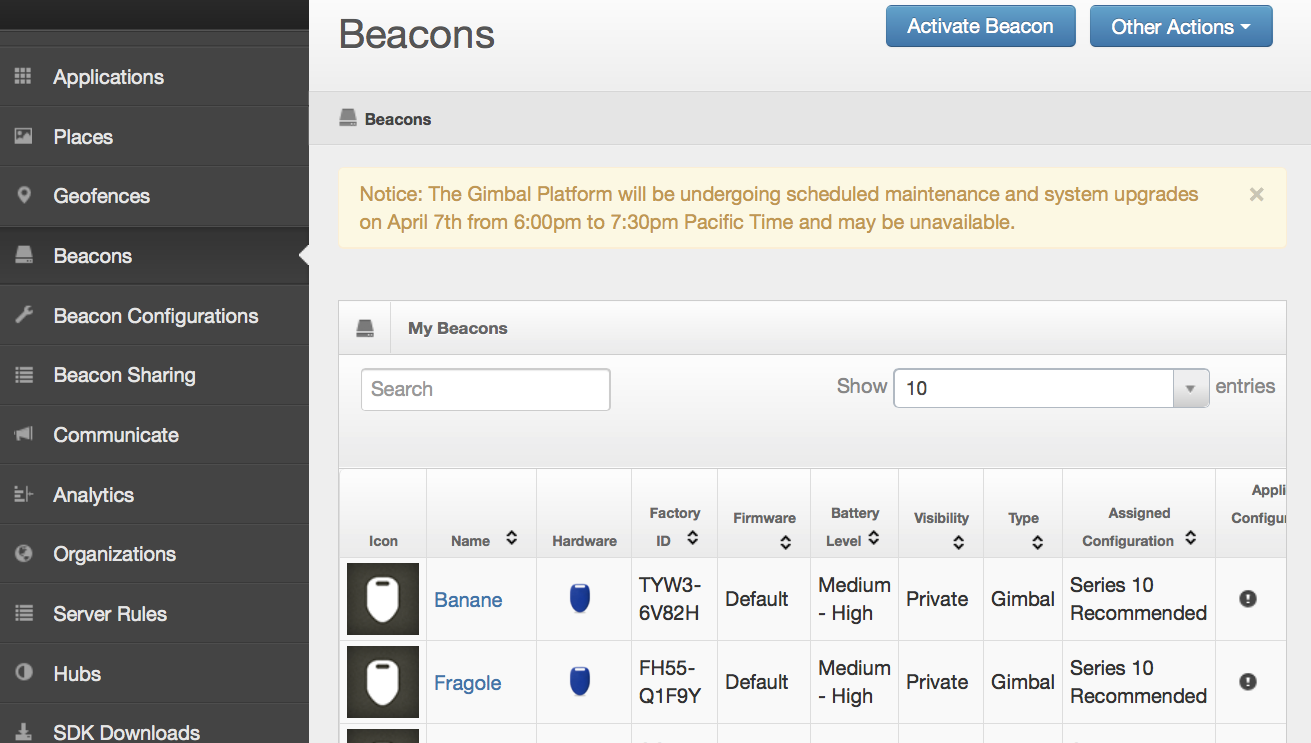
\includegraphics[width=\textwidth]{beacons.png}}
\caption{La schermata contenente il listato dei beacon nel portale Gimbal}
\label{fig:beacons}
\end{figure}

\item Selezionare il bottone Activate Beacon
\item Aprire un trasmettitore Gimbal e trovare il Factory ID (per come trovare il Factory ID, vedi figura \ref{fig:factoryid})

\begin{figure}[h!]
\centering{
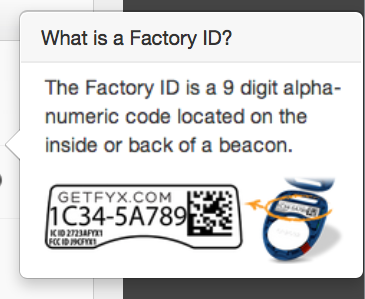
\includegraphics[width=\textwidth]{factoryid.png}}
\caption{Il factory ID di un beacon}
\label{fig:factoryid}
\end{figure}

\item Inserire come nome del Beacon l’ingrediente esattamente come riportato nell’ElencoIngredienti (fornito di seguito) e il Factory ID (vedi figura \ref{fig:activate-beacon})

\begin{figure}[h!]
\centering{
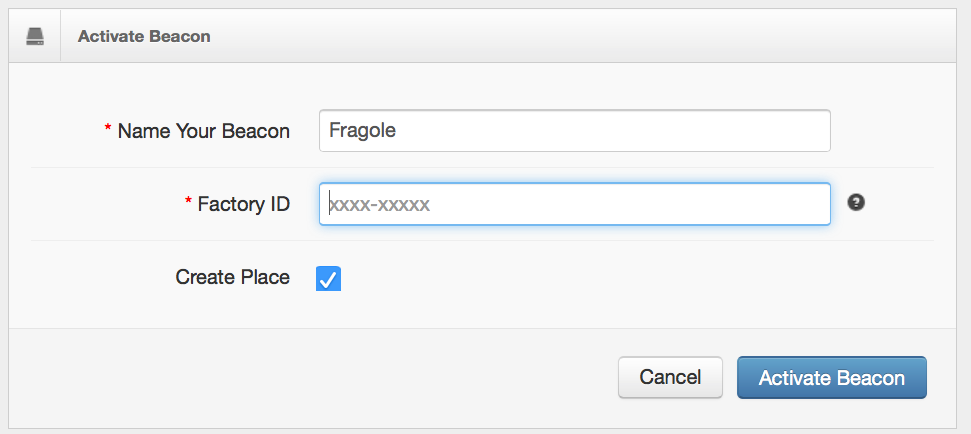
\includegraphics[width=\textwidth]{activate-beacon.png}}
\caption{Schermata di attivazione di un beacon nel portale Gimbal}
\label{fig:activate-beacon}
\end{figure}

\item Confermare con Activate Beacon
\item Ripetere per tutti i trasmettiri/ingredienti
\end{enumerate}

\subsection{Elenco Ingredienti}
\begin{itemize}
\item Ciliegie
\item Mirtilli
\item Uova
\item Pomodori
\item Insalata verde
\item Piselli
\item Zucchero
\item Zucchine
\item Banane
\item Gamberi
\item Mele
\item Kiwi
\item Riso
\item Fagioli
\item Farina
\item Latte
\item Peperoni
\item Pasta
\item Mozzarella
\item Fragole
\item Mango
\item Carote
\item Pollo
\item Ceci
\item Cetrioli
\item Cipolle
\end{itemize}

\subsection{Il gioco}
\subsubsection{Schermata Iniziale e principi generali}

\begin{figure}[h!]
\centering{

\includegraphics[width=\textwidth]{splash.png}}
\caption{Lo splash screen di Chef per un Giorno}
\label{fig:splash}
\end{figure}

La prima schermata (vedi figura \ref{fig:splash}) permette di scegliere tra la modalità singola o multipla. In basso al centro della schermata è anche possibile inserire un indirizzo mail per l’invio dei dati di gioco. Per tornare indietro a questa schermata dalla altre è necessario selezionare il pulsante indietro nella barra inferiore (indicato con un triangolo orientato verso sinistra). 
Il tavolo di gioco comprende il dispositivo Android e uno spazio dove appoggiare i trasmettitori.
Prima di preparare qualsiasi piatto allontanare tutti i trasmettitori dal tavolo di gioco.

\subsubsection{Modalità Singola}

Se si seleziona modalità singola comparirà la schermata di selezione dei piatti (vedi figura \ref{fig:screen1}). È possibile scegliere due o quattro piatti da preparare. Dopo averli selezionati cliccare il tasto Ok per continuare. In alternativa è possibile generale una partita con piatti casuali (è casuale anche il numero di piatti) schiacciando il tasto Casuale.
Dopo la scelta dei piatti comparirà la schermata di gioco principale (vedi figura \ref{fig:screen2}). A sinistra in alto comparirà il piatto da preparare, sotto di questo, se il piatto appartiene al Livello 1, appariranno anche tante pentole arancioni quanti sono il numero degli ingredienti. Se il piatto appartiene al Livello 2 non comparirà nulla. 
Avvicinando un trasmettitore al tavolo di gioco comparirà una pentola verde se l’ingrediente appartiene al piatto, rossa se non appartiene. La pentola rossa indica che c’è almeno un ingrediente errato (possono essere anche due, tre, e così via) e scomparirà quando tutti gli ingredienti errati saranno allontanati dal tavolo di gioco. Un piatto è completato quando vengono avvicinati tutti gli ingredienti corretti e nessuno errato.
Una volta completato il piatto, questo verrà aggiunto alla tavola e verrà mostrato il nuovo piatto da preparare. Quando tutti i piatti sono preparati il gioco è terminato. Per tornare alla schermata principale cliccare il tasto indietro di Android.

\begin{figure}[h!]
\centering{
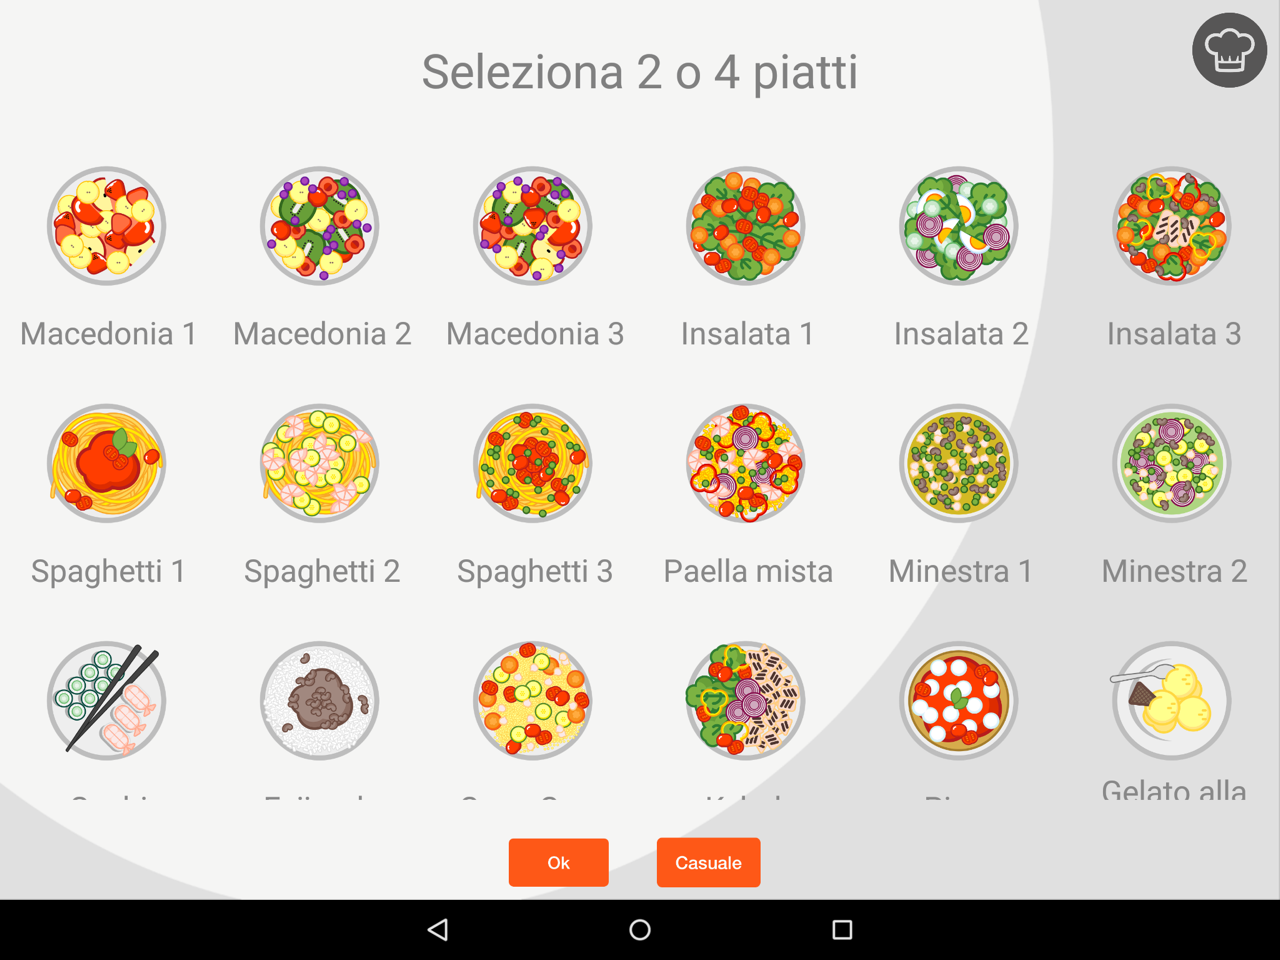
\includegraphics[width=\textwidth]{screen1.png}}
\caption{La schermata di selezione dei piatti}
\label{fig:screen1}
\end{figure}

\begin{figure}[h!]
\centering{
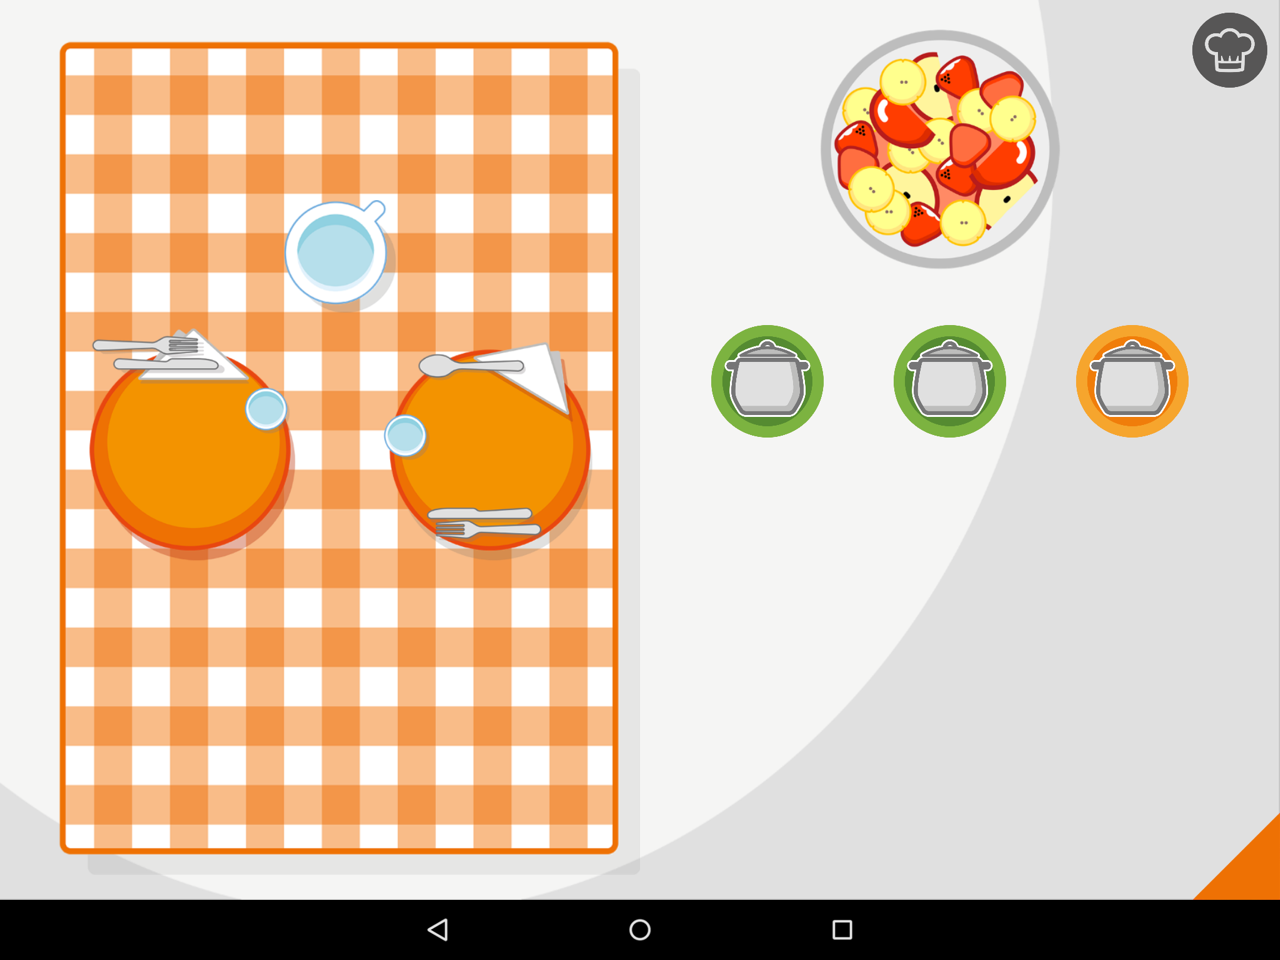
\includegraphics[width=\textwidth]{screen2.png}}
\caption{La schermata di gioco in modalità single player}
\label{fig:screen2}
\end{figure}


\subsubsection{Modalità Multiplayer}
È molto simile alla modalità singola con le seguenti varianti:
\begin{itemize}
\item I due dispositivi devono essere connessi alla stessa rete Wi-Fi
\item I due tavoli di gioco devono essere lontani l’uno dall’altro per evitare interferenze
\item Prima della selezione dei piatti è necessario che su un dispositivo si selezioni Crea una partita e sull’altro Entra in una partita
\item È obbligatorio selezionare quattro piatti (2 per squadra)
\item I quattro piatti verrano scelti dal dispositivo che crea la partita, l’altro rimarrà in attesa fino a selezione avvenuta
\item Giocano due squadre quella arancione e quella viola, il colore della squadra è indicato nella schermata di gioco dal colore presente nell’angolo in basso a destra.
\item Quando un piatto è completato da una squadra, questo compare anche nella tavola della squadra avversaria
\item Se su uno dei due dispositivi esce dal gioco, anche l’altro abbandonerà il gioco
\end{itemize}
In figura \ref{fig:screen3} è mostrata la schermata di gioco in modalità multiplayer.

\begin{figure}[h!]
\centering{
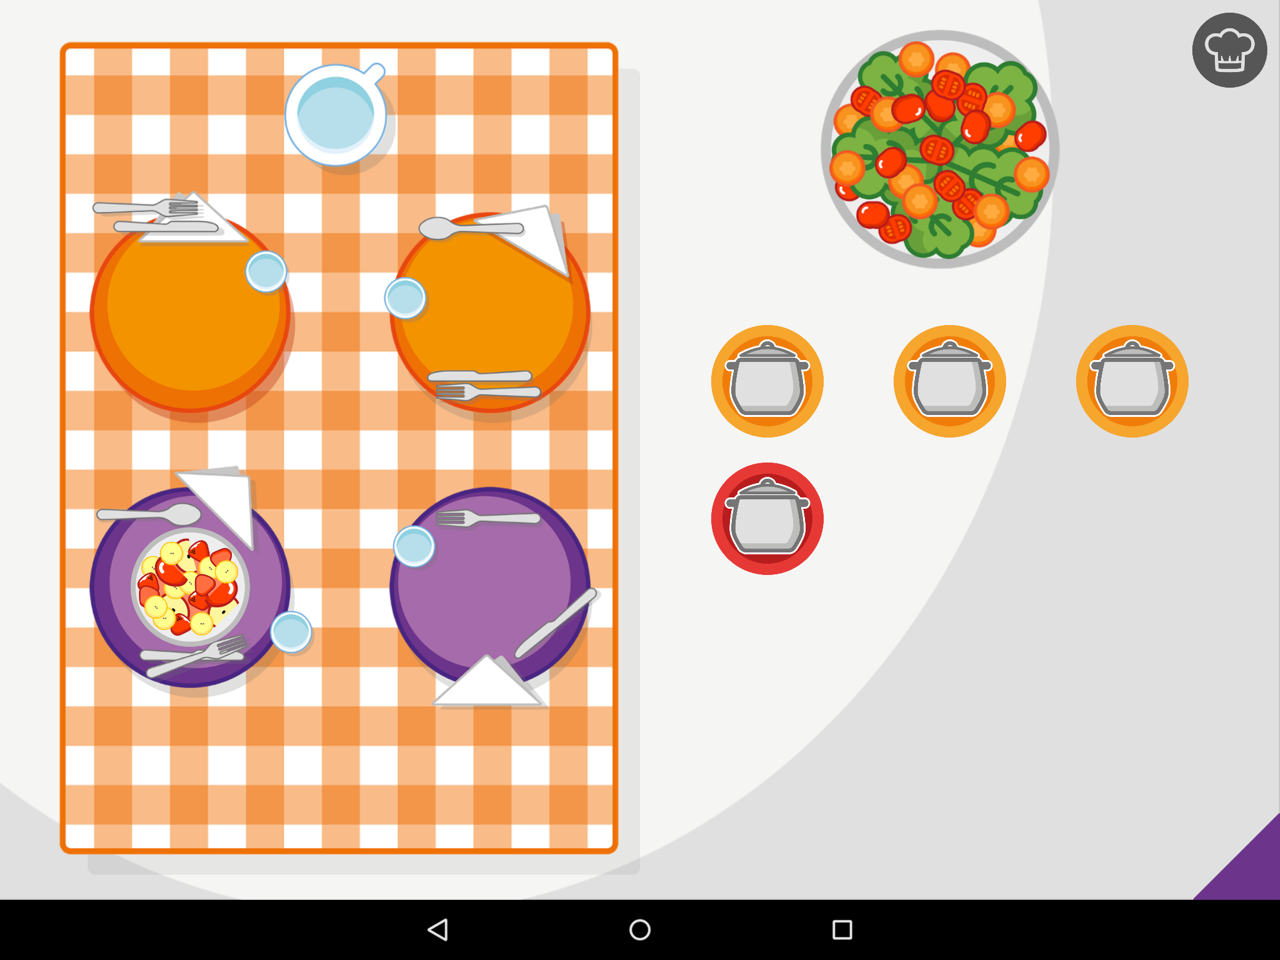
\includegraphics[width=\textwidth]{screen3.png}}
\caption{La schermata di gioco in modalità multiplayer}
\label{fig:screen3}
\end{figure}

\subsubsection{Invio dei dati di gioco}

Se è stata inserita una mail valida (vedi Schermata Principale) verrà inviata una mail con i seguenti dati per ogni piatto realizzato:

\textless nome del piatto\textgreater, \textless timestamp inizio\textgreater, \textless timestamp fine\textgreater, \textless durata in secondi\textgreater, \textless ingredienti in ordine di rilevazione\textgreater, \textless errori\textgreater

Es:

Macedonia 1, 1428877207567, 1428877307567, 100, Mele, Fragole, Banane, errors(Carote, Pomodori)
